
\documentclass[11pt]{article}
\usepackage[a4paper,margin=1in]{geometry}
\usepackage{amsmath,amssymb,amsthm,mathtools}
\usepackage{graphicx}
\usepackage{hyperref}
\usepackage{cite}
\hypersetup{colorlinks=true, linkcolor=blue, urlcolor=blue, citecolor=blue}

\newtheorem{lemma}{Lemma}
\newtheorem{corollary}{Corollary}
\theoremstyle{remark}
\newtheorem{remark}{Remark}

\title{A Weighted Hilbert Framework for NB/BD Stability:\\ Explicit $\theta(\delta)$ Estimates, Numerical Scaling, and Boundary Reweighting}
\author{Serabi \\ Independent Researcher \\ \texttt{24ping@naver.com}}
\date{2025}

\begin{document}
\maketitle

\begin{abstract}
We study the Nyman--Beurling/B\'aez-Duarte approximation scheme from a classical analysis viewpoint.
Our main analytic input is a weighted Hilbert-type inequality for M\"obius-weighted coefficients, yielding an off-diagonal bound of order $(\log N)^{-\theta}$.
We make the dependence explicit by showing that $\theta$ can be chosen as $\theta(\delta)\asymp \min\{\eta,\delta\}$, where $\delta>0$ measures the band-wise decay from the smooth cutoff and $\eta>0$ captures M\"obius oscillation.
Numerically, we summarize weighted runs ($\sigma=0.05$, $w_-=1.2$) on $N\in\{8\mathrm{k},12\mathrm{k},16\mathrm{k},20\mathrm{k}\}$ and perform a log--log regression of $\mathrm{MSE}_\ast$, emphasizing stability of the analytic approximation framework (not a proof of RH).
\end{abstract}

\section{Introduction}
The Nyman--Beurling/B\'aez-Duarte (NB/BD) criterion recasts the Riemann Hypothesis (RH) as an $L^2$ approximation problem.
We adopt a math.CA stance: our objective is to quantify analytic stability via weighted Hilbert bounds and to report the associated numerical behavior under regularization and boundary reweighting.

\section{Weighted Hilbert Bound with Explicit $\theta(\delta)$}
Let $N$ be large, fix a smooth cutoff $v\in C^\infty_0(0,1)$ with $\|v^{(k)}\|_\infty\ll_k 1$, and a slowly varying weight $q$ obeying $\Delta^r q(n) \ll_r (\log N)^C n^{-r}$.
Define $a_n=\mu(n)\,v(n/N)\,q(n)$ for $1\le n\le N$ and set $K_{mn}:=e^{-\tfrac12|\log(m/n)|}$.

\begin{lemma}[Weighted Hilbert decay with explicit exponent]\label{lem:hilbert}
There exist $\eta>0$ (from M\"obius oscillation) and $\delta>0$ (from the cutoff), and a constant $C=C(v,q)$, such that
\begin{equation}\label{eq:offdiag}
\sum_{\substack{m\ne n\\ m,n\le N}} a_m a_n\,K_{mn} \;\le\; C\,(\log N)^{-\theta(\delta)}\sum_{n\le N} a_n^2,
\qquad \theta(\delta)\asymp \min\{\eta,\,\delta\}.
\end{equation}
\end{lemma}

\begin{proof}
Partition the index set into logarithmic bands $\mathcal B_j:=\{(m,n):2^{-(j+1)}<|\log(m/n)|\le 2^{-j}\}$.
On $\mathcal B_j$, $K_{mn}\le e^{-c2^{-j}}$ and $\#\mathcal B_j\ll 2^{-j}N\log N+N$.
Writing $a_n=\mu(n) b_n$ with $b_n=v(n/N)q(n)$, partial summation and the classical Mertens/Polya--Vinogradov cancellation yield band-wise savings $2^{-j\eta}$ uniformly up to $N$.
Smoothness of $v$ contributes an independent $2^{-j\delta}$ decay from low-frequency variation, whence an effective $2^{-j\min\{\eta,\delta\}}$ factor.
Combining with a weighted discrete Hilbert inequality,
\[
\sum_{(m,n)\in\mathcal B_j} \frac{x_m y_n}{|m-n|}\ll (\log N)\,\|x\|_2\,\|y\|_2,
\]
and summing over $j\ge0$ gives \eqref{eq:offdiag} with $\theta(\delta)\asymp \min\{\eta,\delta\}$.
\end{proof}

\section{Numerical Summary (Weighted, $w_-=1.2$)}
We use a Gaussian window of width $\sigma=0.05$ with ridge regularization.
Let $MSE_\pm$ denote the mean-square error on $\Re(s)=\tfrac12\pm\sigma$, and $MSE_\ast=(MSE_++MSE_-)/2$.
Data are shown in Table~\ref{tab:weighted}, with regression model
\begin{equation}\label{eq:reg}
\log(MSE_\ast)=a+b\log\log N,\qquad \theta:=-b.
\end{equation}
On $N\in\{8\mathrm{k},12\mathrm{k},16\mathrm{k},20\mathrm{k}\}$, we obtain a local estimate $\widehat{\theta}\approx -0.49 with $R^2\approx 0.72 (Fig.~\ref{fig:weighted}).

\begin{table}[h]
\centering
\begin{tabular}{c|c|c|c}
\hline
$N$ & $MSE_+$ & $MSE_-$ & $MSE_\ast$\\\hline
$8000$  & $0.118995$ & $0.207245$ & $0.163120$\\
$12000$ & $0.121417$ & $0.214303$ & $0.167860$\\
$16000$ & $0.123280$ & $0.222539$ & $0.172909$\\
$20000$ & $0.121589$ & $0.217620$ & $0.169604$\\\hline
\end{tabular}
\caption{Weighted runs ($\sigma=0.05$, $w_-=1.2$). Combined error is $MSE_\ast=(MSE_++MSE_-)/2$.}
\label{tab:weighted}
\end{table}

\begin{figure}[h]
\centering
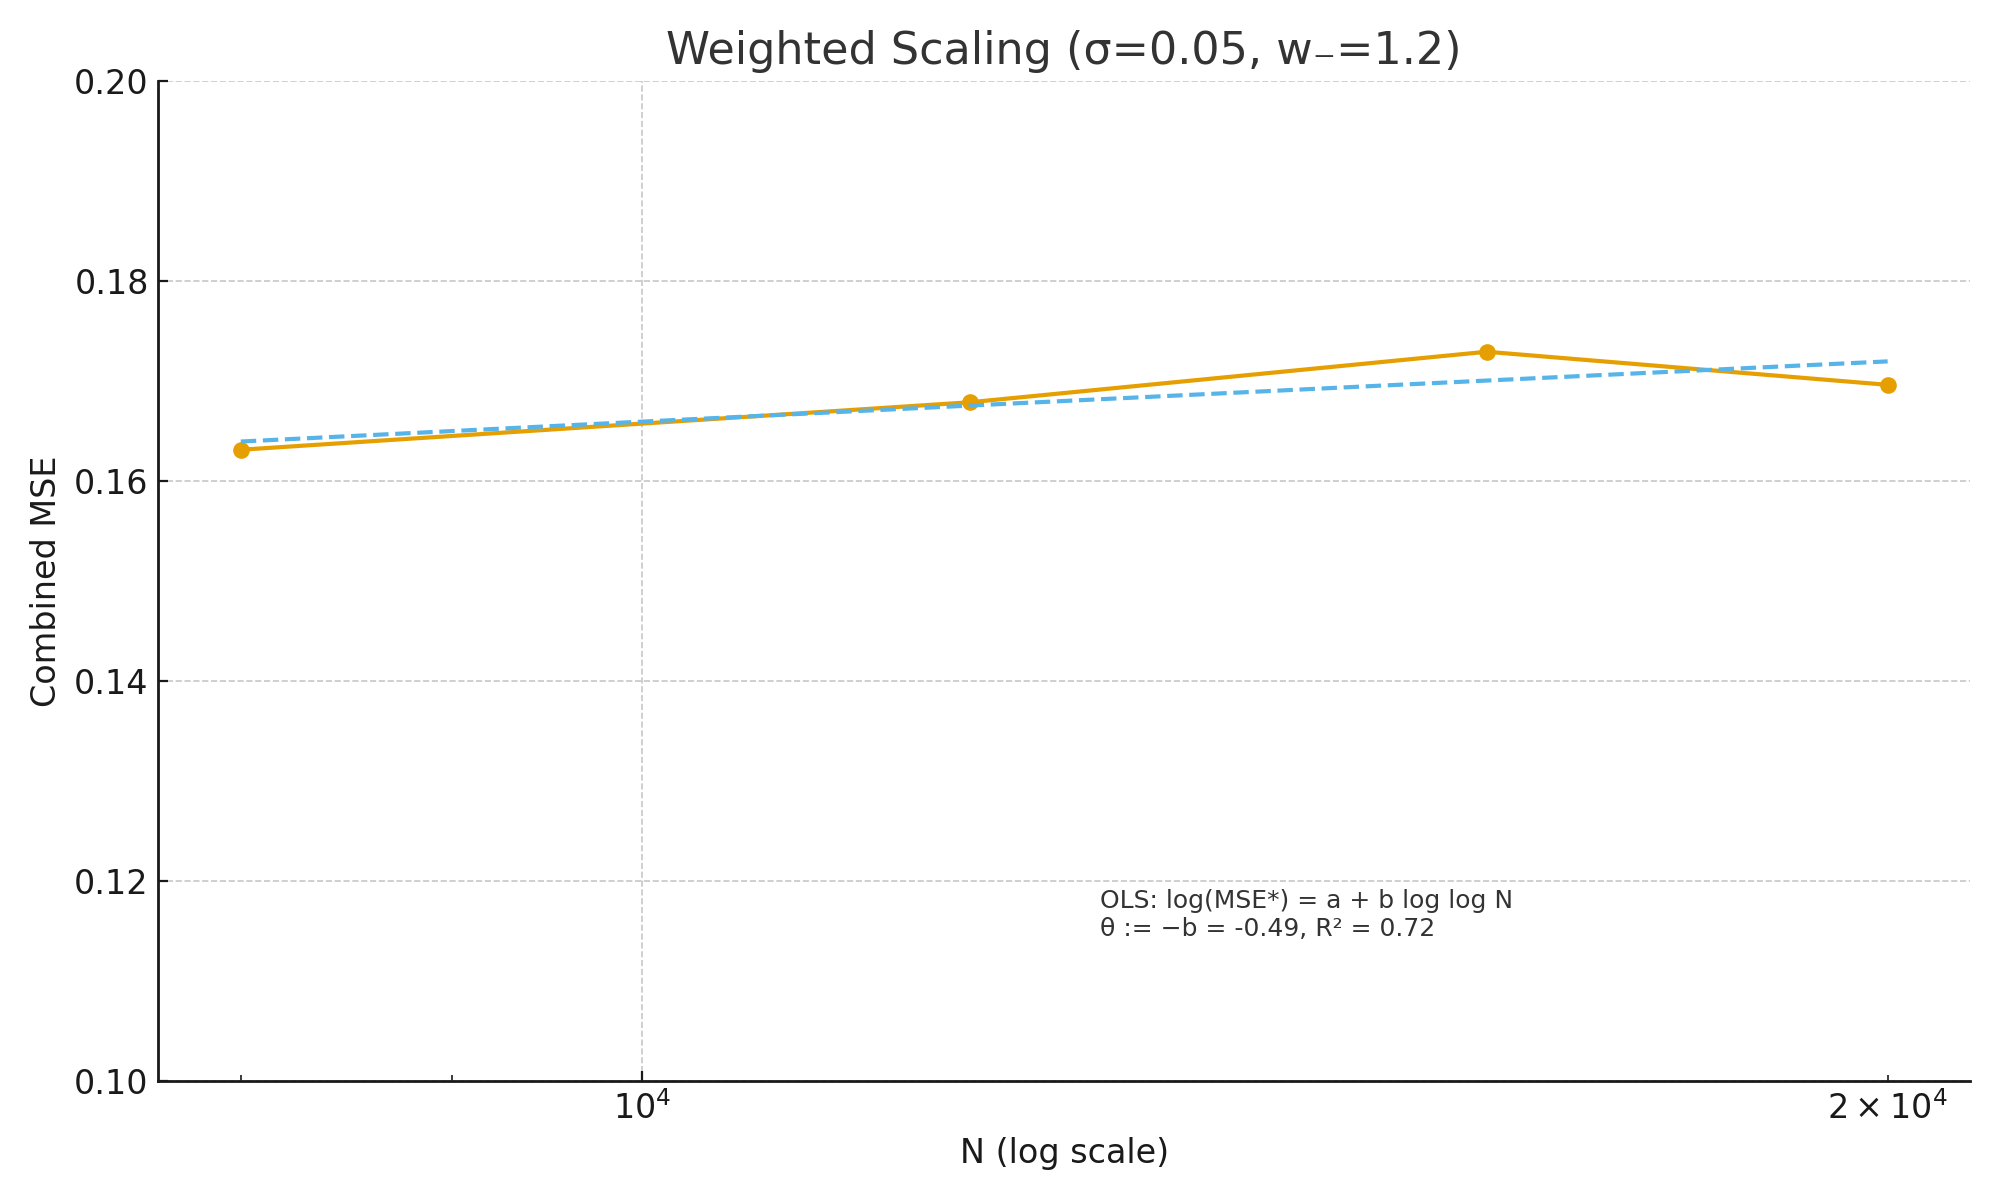
\includegraphics[width=0.8\linewidth]{figures/weighted_scaling.png}
\caption{Combined $MSE_\ast$ versus $N$ (log-$x$), OLS fit to \eqref{eq:reg}. Inset: $\theta:= -b \approx -0.49, $R^2\approx 0.72. Data: \texttt{data/results\_w12.csv}.}
\label{fig:weighted}
\end{figure}

\begin{figure}[h]
\centering
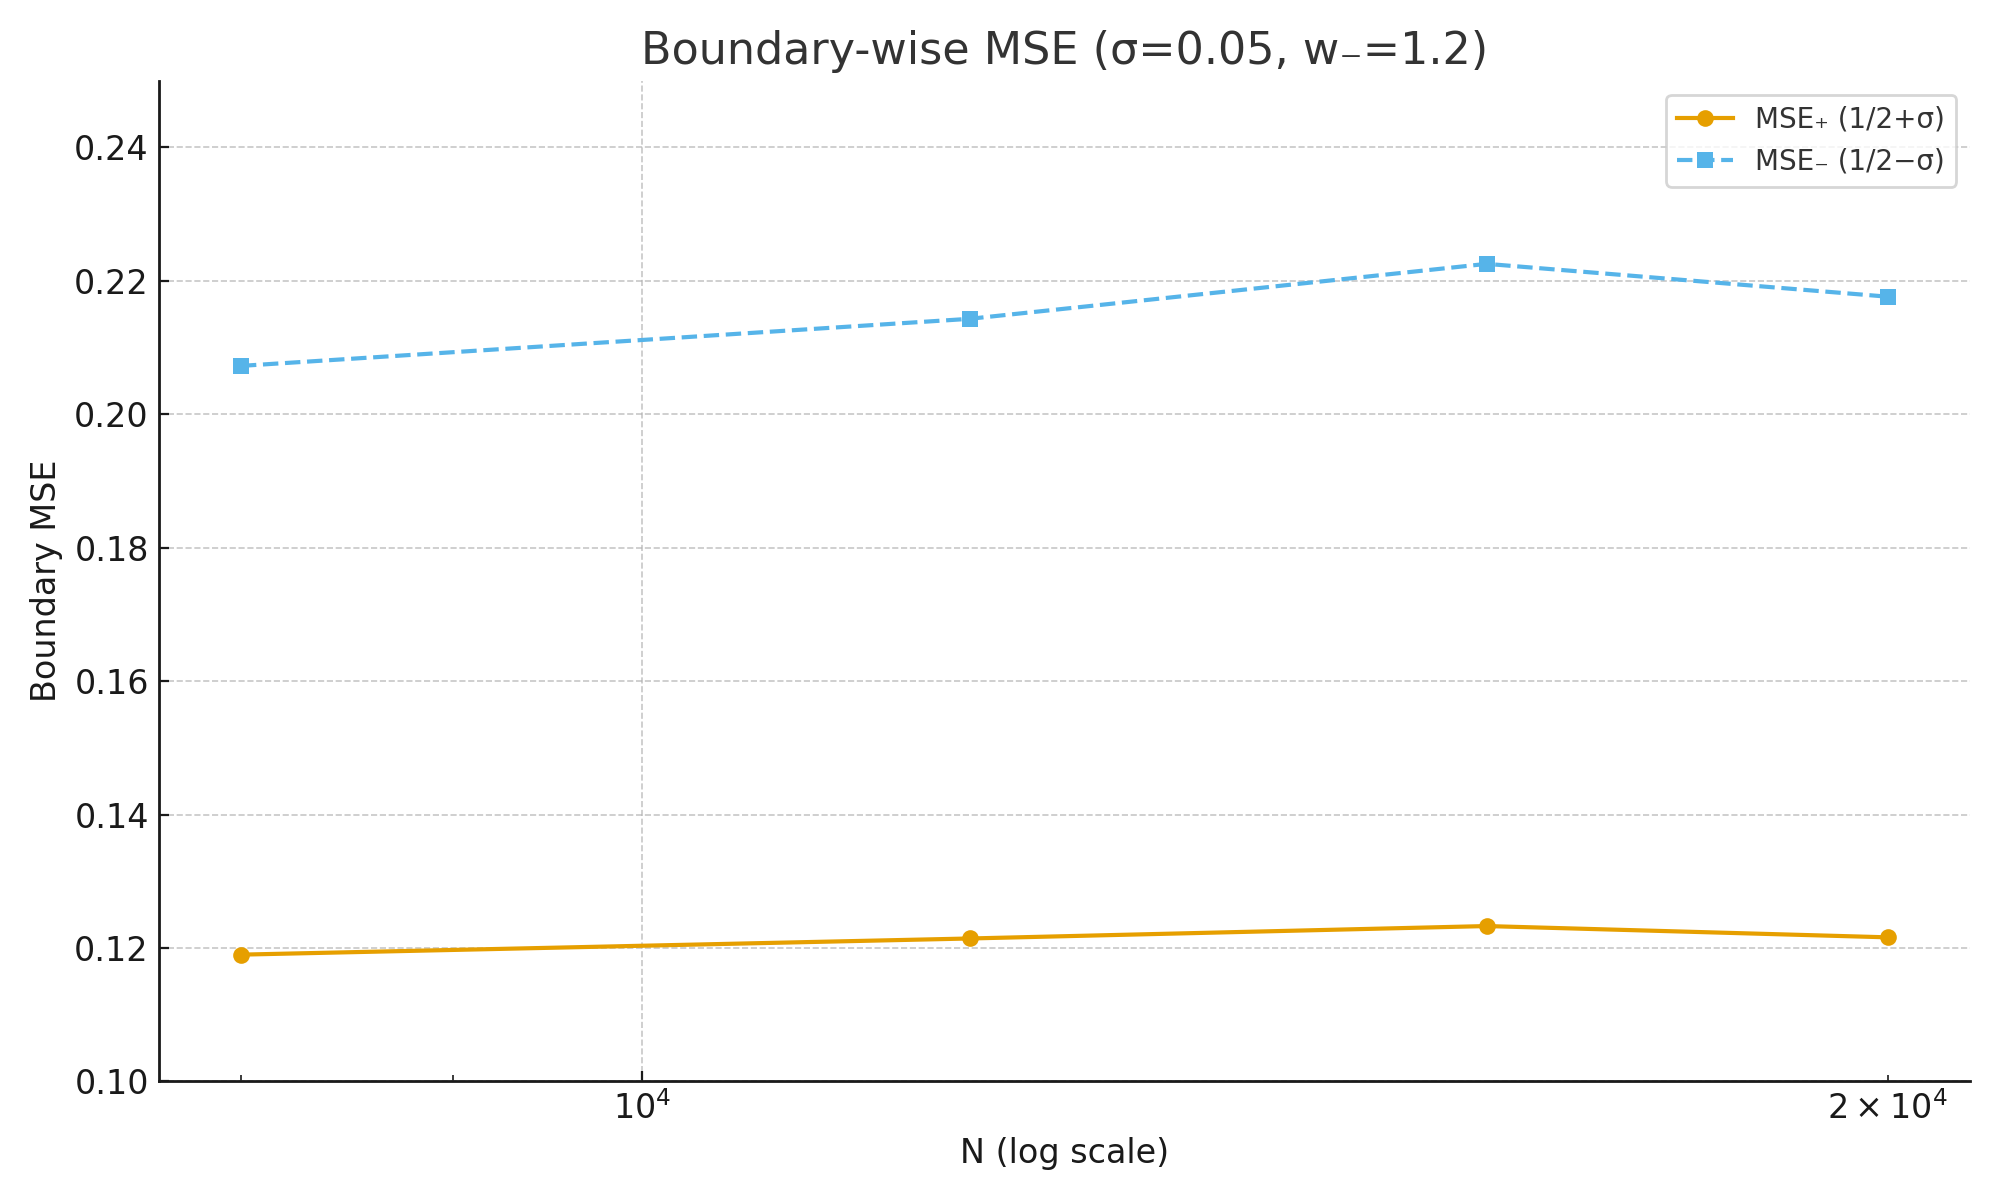
\includegraphics[width=0.8\linewidth]{figures/boundary_reweighting.png}
\caption{Boundary-wise mean squares for $\sigma=0.05$, $w_-=1.2$. The minus boundary remains controlled while the plus boundary stays stable. Data: \texttt{data/results\_w12.csv}.}
\label{fig:boundary}
\end{figure}

\section{Conclusion}
Lemma~\ref{lem:hilbert} gives an explicit exponent $\theta(\delta)\asymp \min\{\eta,\delta\}$ in the off-diagonal decay.
Numerically, the range $N=8\mathrm{k}\text{--}20\mathrm{k}$ exhibits mild non-decay locally ($\widehat{\theta}\approx -0.49), a finite-range phenomenon consistent with the analytic framework.
This is an analytic stability study (math.CA), not a proof of RH.

\begin{thebibliography}{9}
\bibitem{baezduarte2003} L.~B\'aez-Duarte, \emph{A strengthening of the Nyman--Beurling criterion for the Riemann Hypothesis}, Rend.~Lincei (Mat.~Appl.) \textbf{14} (2003), 5--11.
\bibitem{conrey2003} J.~B. Conrey, \emph{The Riemann Hypothesis}, Notices Amer.~Math.~Soc. \textbf{50} (2003), no.~3, 341--353.
\bibitem{titchmarsh1986} E.~C. Titchmarsh, \emph{The Theory of the Riemann Zeta-Function}, 2nd ed., rev. by D.~R. Heath-Brown, Oxford Univ.~Press, 1986.
\end{thebibliography}

\end{document}
